\documentclass[10pt,journal]{IEEEtran}
\usepackage[utf8]{inputenc}
\usepackage[T1]{fontenc}
\usepackage{graphicx}
\graphicspath{{analysis/}}
\usepackage{amsmath}
\usepackage{booktabs}
\usepackage{multirow}
\usepackage{tikz}
\usetikzlibrary{shapes.geometric, arrows.meta, positioning, calc}
\usepackage{url}
\usepackage{hyperref}
\hypersetup{colorlinks=true, linkcolor=blue, citecolor=blue, urlcolor=blue}

% Number only sections (I, II, ...) and subsections (A, B, ...); this stops
% IEEEtran from printing broken run-in heading numbers like "1.0.0.1".
\setcounter{secnumdepth}{3}

\begin{document}

\title{Quantifying and Forecasting the Impact of the 2025 U.S.\ Government
Shutdown on New York--Metro Flight Delays}

\author{Pranish~Uprety\\
Department of Computer Science, Caldwell University\\
\textit{Advisor:}~Dr.~Sushil~Poudel}

\maketitle

\begin{abstract}
The 43-day 2025 federal government shutdown strained air-traffic-controller
staffing and culminated in an FAA emergency order cutting flights at 40 major
airports. We quantify its impact on the New York metropolitan airports (EWR,
JFK, LGA) using Bureau of Transportation Statistics on-time records, and we
test whether the impact could have been forecast. Comparing October--November
2025 against the same months of 2024, mean departure delay rose 107\% at JFK
and 149\% at LaGuardia (both $p<10^{-4}$ on daily means) and 27\% at Newark
(not significant, $p=0.069$), while cancellation rates rose three- to
eight-fold, exceeding 4\% of scheduled flights after the FAA order. Three
independent counterfactuals (a prior-year baseline, a machine-learned
normal-operations model, and the same model with METAR weather controls) agree
that the shutdown produced roughly $0.40$--$0.42$ million excess departure-delay
minutes at the three airports, about \$41M at the industry cost of
\$100.76 per block-minute; weather explains essentially none of it. A
forecasting model using only information available in advance (calendar,
scheduled traffic, and a shutdown indicator) predicts the held-out November
2025 disruption better than a normal-year climatology at all three airports
($R^2$ 0.12--0.23 versus $\le 0.09$). Finally, we document that inter-airport
delay coupling is \emph{state-dependent}: the correlation between Newark's
delay and JFK's delay one hour later is $r\!=\!0.55$--$0.57$ during disrupted
periods (the shutdown; January 2023, containing the NOTAM outage) but only
$r\!=\!0.19$ in normal operations. These results provide a reproducible,
weather-controlled measurement of the shutdown's local aviation cost and
motivate graph-based intervention models that activate under disruption.
\end{abstract}

% =====================================================================
\section{Introduction}
\label{sec:intro}
\IEEEPARstart{F}{light} delays are a persistent, costly feature of the U.S.\
National Airspace System: industry estimates place the direct operating cost of
delay at \$100.76 per block-minute for calendar year 2024 \cite{a4a2025}, and
system-wide costs in the tens of billions of dollars annually. Delays are also
not independent events. Airports are coupled through shared aircraft, crews,
and controlled airspace, so a disruption at one hub ripples outward
\cite{fleurquin2013}.

The 2025 federal government shutdown provided a rare, well-documented natural
experiment in system-wide disruption. Beginning October~1, 2025 and lasting 43
days, it forced air-traffic controllers to work unpaid, drove staffing
shortfalls, and culminated in an FAA emergency order (November~6, 2025)
mandating traffic reductions at 40 ``High-Impact Airports'' \cite{faa2025order}.
A Federal Reserve Bank of Richmond difference-in-differences study estimated
roughly one million extra delay work-hours nationwide (about \$66M)
\cite{richmondfed2025}, and a policy analysis attributed a multi-billion-dollar
economic hit to the blanket cuts, arguing for targeted, data-driven
interventions instead \cite{ctp2026}.

We study the shutdown's effect on the New York metropolitan sub-network
(Newark EWR, Kennedy JFK, LaGuardia LGA), the most congested and operationally
coupled metro system in the country. We frame the study around three questions:

\begin{enumerate}
  \item \textbf{Measurement.} How large was the shutdown's effect on
        departure delays and cancellations, and is it statistically
        distinguishable from normal year-to-year variation?
  \item \textbf{Attribution.} Does the effect survive a weather control, or
        could the 2025 excess reflect worse weather rather than the shutdown?
  \item \textbf{Forecastability.} Could the disruption have been predicted in
        advance from public information, without peeking at realized delays?
\end{enumerate}

\paragraph{Objective}
The objective of this work is to deliver a reproducible, weather-controlled,
and \emph{forecastable} measurement of the 2025 shutdown's impact on NYC-metro
departure delays, expressed in both delay-minutes and dollars, and to
characterize how the metro's inter-airport delay coupling changes under
disruption, thereby establishing the empirical foundation for
disruption-aware, intervention-capable graph models of the airspace.

\paragraph{Contributions}
(i)~A reproducible measurement of the shutdown's impact on NYC-metro
departures: +107\% mean delay at JFK and +149\% at LGA (both significant at
$p<10^{-4}$), +27\% at EWR (not significant), and cancellation rates rising
from under 1\% to over 4\% after the FAA order.
(ii)~Three converging counterfactual estimates of the excess delay
(prior-year baseline; a gradient-boosted normal-operations model; the same
model with METAR weather features), all in the range 0.40--0.42 million
delay-minutes ($\approx$\,\$41M), with weather explaining essentially none of
the excess.
(iii)~An honest, leakage-free forecasting test showing a shutdown-aware model
beats climatology on the unseen November 2025 period.
(iv)~Evidence that inter-airport delay coupling in the metro sub-network is
state-dependent, strengthening sharply under disruption, an empirical
motivation for intervention-aware graph models, which we outline as future
work.
All code, data provenance, and exact figures in this paper are reproducible
from public BTS and Iowa Environmental Mesonet (IEM) archives with the scripts
accompanying this paper.

% =====================================================================
\section{Related Work}
\label{sec:related}
Our study sits at the intersection of three strands of prior work: graph-based
delay prediction, causal and benchmark studies of delay, and empirical
analyses of real-world disruptions. Table~\ref{tab:related} summarizes the
predictive and causal models; we then discuss each strand.

\begin{table}[!t]
\centering
\small
\caption{Representative prior work on graph-based delay modeling and the gap
each leaves open for intervention-aware measurement.}
\label{tab:related}
\begin{tabular}{p{1.7cm}p{2.6cm}p{1.7cm}}
\toprule
Study & Approach & Open gap \\
\midrule
Cai 2023 \cite{cai2023} & Geographical+operational GCN & Observational only \\
Zeng 2021 \cite{zeng2021} & Time-evolving graph DL & Static thresholds \\
Jiang 2022 \cite{jiang2022} & Multi-task local--global GNN & No counterfactuals \\
Guo 2020 \cite{guo2020} & Dual-attention ST-GNN & No intervention \\
Vasana 2025 \cite{vasana2025} & Cause-inferring ST-GNN & Diagnostic only \\
Zhu 2024 \cite{zhu2024} & CausalNet (Granger graph) & Not interventional \\
Tang 2026 \cite{tang2026} & Edge-based GNN & Representation only \\
Franco 2026 \cite{franco2026} & GAT/CatBoost holdings & Class imbalance \\
Xu 2025 \cite{xu2025} & Aeolus benchmark & No intervention tasks \\
\bottomrule
\end{tabular}
\end{table}

\paragraph{Graph models for delay prediction}
Graph neural networks dominate recent delay-prediction work. Cai et al.\
separate geographical and operational graph structure with dual aggregators
(GOGCN), outperforming plain GCNs but remaining strictly observational
\cite{cai2023}. Zeng et al.\ track topological shifts through time-evolving
graphs as disruptions propagate, at high computational cost and with static
delay-state thresholds \cite{zeng2021}. Jiang et al.\ balance local node
features against macro network constraints in a multi-task local--global
network but cannot predict unobserved counterfactual outcomes \cite{jiang2022}.
Guo et al.'s SGDAN embeds graph- and sequence-level attention for advance
departure-delay forecasts, again as pure prediction \cite{guo2020}. More recent
work separates local from cascading delays and infers delay \emph{causes}
\cite{vasana2025} and frames the operational cost trade-off of delay explicitly
\cite{kim2024}, but stops at diagnosis rather than prescription.

\paragraph{Causal, edge-centric, and benchmark studies}
The closest model to a causal treatment is CausalNet, which learns a dynamic
Granger-causal graph to drive message passing \cite{zhu2024}; however, Granger
causality is statistical predictive causation, not the interventional
``do-operator'' causation needed to evaluate a ground hold. Edge-centric
formulations improve operational fidelity with delay width/strength metrics
\cite{tang2026} and target specific anomalies such as holding maneuvers, where
tree models with network-centrality features can beat attention networks under
severe class imbalance \cite{franco2026}. The Aeolus benchmark standardizes
leakage-free, multi-modal evaluation but contains no intervention or
counterfactual tasks \cite{xu2025}. Classical network science first established
that delays propagate systemically across the U.S.\ airport network
\cite{fleurquin2013}, the phenomenon our coupling analysis
(Section~\ref{sec:res-coupling}) revisits under disruption.

\paragraph{The 2025 shutdown and prior disruptions}
The Richmond Fed brief \cite{richmondfed2025} is the closest quantitative work:
a difference-in-differences design over 76 million flight operations at 82
airports, controlling for NOAA weather, attributing $\sim$1M extra delay
work-hours ($\sim$\$66M) to the shutdown nationwide. A policy analysis reports
$>$9{,}000 cancellations, $>$6M affected passengers, and a $\sim$\$7.25B
economic hit, arguing that the FAA's blanket 10\% cuts were blunt and that
targeted, data-driven strategies are preferable \cite{ctp2026}. Our study is
complementary: we zoom into the NYC metro, use per-airport-hour counterfactual
models rather than a national panel regression, add the cancellation margin,
and test forecastability. Prior disruptions show the same mechanism: in January
2019, a small rise in controller sick leave forced a LaGuardia ground stop with
cascading East-Coast delays \cite{npr2019}, and the January 2023 NOTAM outage
triggered a nationwide ground stop \cite{icao2023notam, dot2023notam} that we
use as an additional disrupted-regime sample.

% =====================================================================
\section{Methodology}
\label{sec:method}

\subsection{Overview and Experimental Setup}
\label{sec:setup}
Figure~\ref{fig:pipeline} shows the end-to-end pipeline. Starting from public
flight and weather archives, we clean and aggregate flights to an
airport--hour panel, then run three analyses on that common panel: (i) a
measurement-and-counterfactual analysis that quantifies the shutdown's excess
delay and dollar cost; (ii) a strict, leakage-free forecasting test; and (iii)
a coupling analysis that compares local-only against network-augmented
predictors across normal and disrupted regimes. The design follows an
evidence-first plan: rather than assert that delay propagates, we compare a
local model against a network model and measure the incremental gain
($\Delta R^2$, MAE) as the unit of evidence.

\begin{figure}[!t]
\centering
\resizebox{\columnwidth}{!}{%
\begin{tikzpicture}[
  node distance=4mm,
  data/.style={draw, fill=blue!8, rounded corners, align=center,
               font=\scriptsize, text width=6.5cm, minimum height=7mm},
  proc/.style={draw, fill=gray!12, rounded corners, align=center,
               font=\scriptsize, text width=6.5cm, minimum height=7mm},
  out/.style={draw, fill=green!10, rounded corners, align=center,
              font=\scriptsize, text width=6.5cm, minimum height=8mm},
  arr/.style={-{Stealth[length=2mm]}, thick}
]
\node[data] (src) {\textbf{Public data.} BTS On-Time records
(Oct--Nov 2024/2025; Jan 2023) $+$ IEM METAR (EWR, JFK, LGA)};
\node[proc, below=of src] (panel) {\textbf{Preprocess.} Filter Northeast
corridor, drop cancellations for delay stats; aggregate to an
\textbf{airport--hour panel} (mean departure delay, flight counts)};
\node[proc, below=of panel] (an) {\textbf{Three analyses.}
(i) counterfactuals: prior-year, ML normal-ops, weather-adjusted;
(ii) leakage-free forecast: calendar $+$ traffic $+$ shutdown flag;
(iii) coupling: local vs.\ network ridge, lead--lag correlation};
\node[out, below=of an] (out) {\textbf{Outcomes.} Delay change $+$
significance; excess delay-minutes $\rightarrow$ cost at \$100.76/min;
forecast skill vs.\ climatology; state-dependent coupling structure};
\draw[arr] (src) -- (panel);
\draw[arr] (panel) -- (an);
\draw[arr] (an) -- (out);
\end{tikzpicture}%
}
\caption{End-to-end methodology: from public archives to delay, cost,
forecast, and coupling outcomes on a shared airport--hour panel.}
\label{fig:pipeline}
\end{figure}

\subsection{Data}
\label{sec:data}
\paragraph{Flight data}
We use the BTS Reporting Carrier On-Time Performance files \cite{btsontime} for
four months: October--November 2024 (normal operations) and October--November
2025 (the shutdown window; the shutdown began October~1 and the FAA order took
effect November~7). We restrict to departures from eight Northeast-corridor
airports (EWR, JFK, LGA, BOS, PHL, DCA, IAD, BWI): 160,383 operated departures
in the 2024 window and 149,426 in 2025. For the propagation analysis we
additionally use January 2023 (75,574 corridor departures). Delay is
\texttt{DepDelayMinutes} (0 for early/on-time departures); cancelled flights are
excluded from delay statistics but analyzed separately as the cancellation
margin.

\paragraph{Aggregation}
Flights are aggregated to an airport--hour panel by scheduled departure hour:
the panel value is the mean departure delay of flights scheduled in that hour.
Hours with no scheduled departures (overnight) are set to zero delay.

\paragraph{Weather}
Hourly METAR observations for EWR, JFK, and LGA (temperature, wind speed,
visibility, precipitation) for both October--November windows, from the IEM
ASOS archive \cite{iemasos}.

\paragraph{Cost of delay}
We convert delay-minutes to dollars at the Airlines for America CY2024 figure
of \$100.76 per block-minute (crew, fuel, maintenance, ownership)
\cite{a4a2025}. This is a direct-operating-cost figure; it excludes passenger
time, so dollar figures below are conservative in that respect.

\subsection{Methods and Algorithms}
\label{sec:algorithms}
\paragraph{Significance testing}
For the raw effect we compare daily mean delays between years with a Welch
$t$-test ($n{=}61$ days per year) and report a bootstrap 95\% confidence
interval of the daily-mean difference.

\paragraph{Counterfactual estimators for excess delay}
The causal quantity of interest is the delay that would \emph{not} have
occurred absent the shutdown. No single counterfactual is beyond criticism, so
we compute three with different failure modes and check convergence:
\begin{enumerate}
  \item \textbf{Prior-year baseline.} Total delay-minutes in the 2025 window
        minus the same total in 2024. Fails if 2025 differs from 2024 for
        reasons other than the shutdown (traffic mix, weather).
  \item \textbf{Model counterfactual.} A gradient-boosted regressor trained on
        2024 airport-hours (own delay lags $t{-}1..t{-}3$, hour, day-of-week,
        corridor-neighbor lags) predicts each 2025 airport-hour's ``normal''
        delay; the excess is
        $\sum_h \max(0,\, y_h - \hat y_h)\cdot n_h$, where $n_h$ is flights
        operated in hour $h$. Adapts to 2025's actual traffic pattern.
  \item \textbf{Weather-adjusted model.} The same model with METAR wind,
        visibility, and precipitation features, so that any delay explainable
        by 2025's weather is absorbed into the counterfactual.
\end{enumerate}

\paragraph{Leakage-free forecasting model}
To test forecastability we impose a strict rule: no realized-delay features of
any airport are used. Features are the calendar (hour, day-of-week), scheduled
departures in the hour, and a binary shutdown indicator (public knowledge on
the day). We train a gradient-boosted regressor on all of October--November
2024 plus October 2025, and forecast November 2025 (unseen, and containing the
FAA-order peak) against a climatology baseline (mean delay by hour and
day-of-week learned from 2024 only). This separation ensures the model cannot
copy recent delays; it must anticipate the disruption from information available
in advance.

\paragraph{State-dependent coupling}
On an hourly panel of the eight corridor airports, for each NYC-metro target we
compare two ridge regressions on a temporal holdout (final 25\% of hours): a
\emph{local} model (own delay at $t{-}1..t{-}3$, hour-of-day) versus a
\emph{network} model adding all corridor neighbors' delays at $t{-}1$. We report
the change in out-of-sample $R^2$ from adding network features, and the
lead--lag Pearson correlation between Newark's delay at hour $t$ and each
downstream hub's delay at $t{+}1$, across three regimes (January 2023, normal
2024, shutdown 2025).

% =====================================================================
\section{Results: Outcomes and Findings}
\label{sec:results}

\subsection{Effect on Delays and its Significance}
\label{sec:res-effect}
Table~\ref{tab:raw} compares the shutdown window with the same months of the
prior year. Mean departure delay roughly doubled at JFK and more than doubled
at LGA; Newark, chronically delayed even in normal operations, rose by a
smaller fraction. The JFK and LGA increases are highly significant (bootstrap
95\% CIs of the daily-mean difference: $[5.3, 12.4]$ and $[7.9, 18.0]$ minutes
respectively); the EWR increase is \emph{not} significant at the 5\% level (CI
$[-0.01, 9.6]$). Figure~\ref{fig:daily} shows the daily trajectory: the two
years track in early October and diverge as the shutdown wears on, with the
largest gaps around the FAA flight-cut order.

\begin{table*}[!t]
\centering
\caption{NYC-metro departures, October--November, 2024 (normal) vs.\ 2025
(shutdown). Delay statistics are over operated (non-cancelled) flights.
$p$-values are Welch $t$-tests on daily mean delays ($n{=}61$ days per year).}
\label{tab:raw}
\begin{tabular}{lcccccc}
\toprule
Airport & Flights '24 & Flights '25 & Mean delay '24 & Mean delay '25 &
Change & $p$ \\
\midrule
EWR & 21{,}796 & 20{,}417 & 13.2 min & 16.8 min & $+27\%$ & $0.069$ \\
JFK & 20{,}801 & 17{,}180 & 7.6 min & 15.7 min & $+107\%$ & $1.4\times10^{-5}$ \\
LGA & 27{,}413 & 22{,}849 & 7.9 min & 19.8 min & $+149\%$ & $7.3\times10^{-6}$ \\
\bottomrule
\end{tabular}
\end{table*}

\begin{figure*}[!t]
\centering
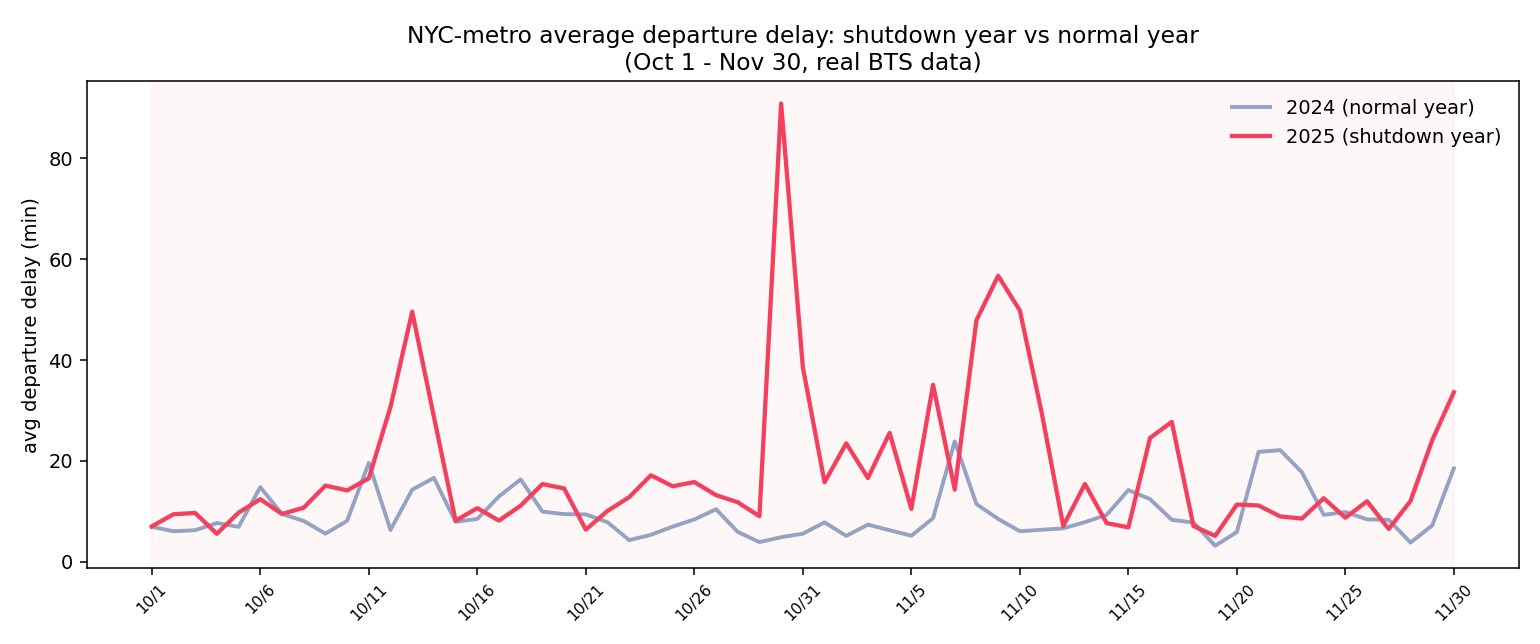
\includegraphics[width=0.9\linewidth]{fig_shutdown_daily.png}
\caption{Daily mean NYC-metro departure delay, shutdown year (2025) vs.\ the
same calendar window in 2024. The gap widens through the shutdown and peaks
around the FAA emergency order of November~6--7.}
\label{fig:daily}
\end{figure*}

\subsection{The Cancellation Margin}
\label{sec:res-cancel}
Delay statistics condition on a flight operating, but the FAA order
\emph{cancelled} flights outright, so delay alone understates the disruption
and suffers survivorship bias. Table~\ref{tab:cancel} quantifies this margin:
cancellation rates rose three- to eight-fold, and after the FAA order reached
3.3--4.9\% of scheduled flights, against essentially zero in the same 2024
dates. In absolute terms the three airports cancelled 1{,}668 flights in the
2025 window versus 339 in 2024.

\begin{table}[!t]
\centering
\small
\caption{Cancellation rates, October--November windows (BTS). ``Post-order''
is November 7 onward (2025) and the same calendar dates in 2024.}
\label{tab:cancel}
\begin{tabular}{lcccc}
\toprule
Airport & Cancel '24 & Cancel '25 & Post-ord.\ '24 & Post-ord.\ '25 \\
\midrule
EWR & 0.74\% & 2.69\% & 0.37\% & 4.85\% \\
JFK & 0.34\% & 2.13\% & 0.01\% & 3.34\% \\
LGA & 0.39\% & 3.10\% & 0.11\% & 4.28\% \\
\bottomrule
\end{tabular}
\end{table}

\subsection{Excess Delay under Three Counterfactuals}
\label{sec:res-excess}
Table~\ref{tab:excess} reports the excess departure delay attributed to the
shutdown under the three estimators of Section~\ref{sec:algorithms}. The three
estimates agree within 5\%. Notably, the weather-adjusted estimate is not
smaller than the others, even though 2025's window was somewhat worse
meteorologically (mean wind 10.1 vs.\ 8.8~kt; roughly double the precipitation
and low-visibility hours). Figure~\ref{fig:counterfactual} shows the actual
delay against the normal-expectation counterfactual, with the shaded
shutdown-attributable excess.

\begin{table}[!t]
\centering
\small
\caption{Excess departure delay attributable to the shutdown, NYC metro,
October--November 2025, under three counterfactuals. Dollars at
\$100.76/block-minute \cite{a4a2025}.}
\label{tab:excess}
\begin{tabular}{lcc}
\toprule
Counterfactual & Excess delay (min) & Cost \\
\midrule
Prior-year (2024) baseline & 401{,}999 & \$40.5M \\
Model (calendar+lags+network) & 409{,}455 & \$41.3M \\
Model + METAR weather & 420{,}837 & \$42.4M \\
\bottomrule
\end{tabular}
\end{table}

\begin{figure*}[!t]
\centering
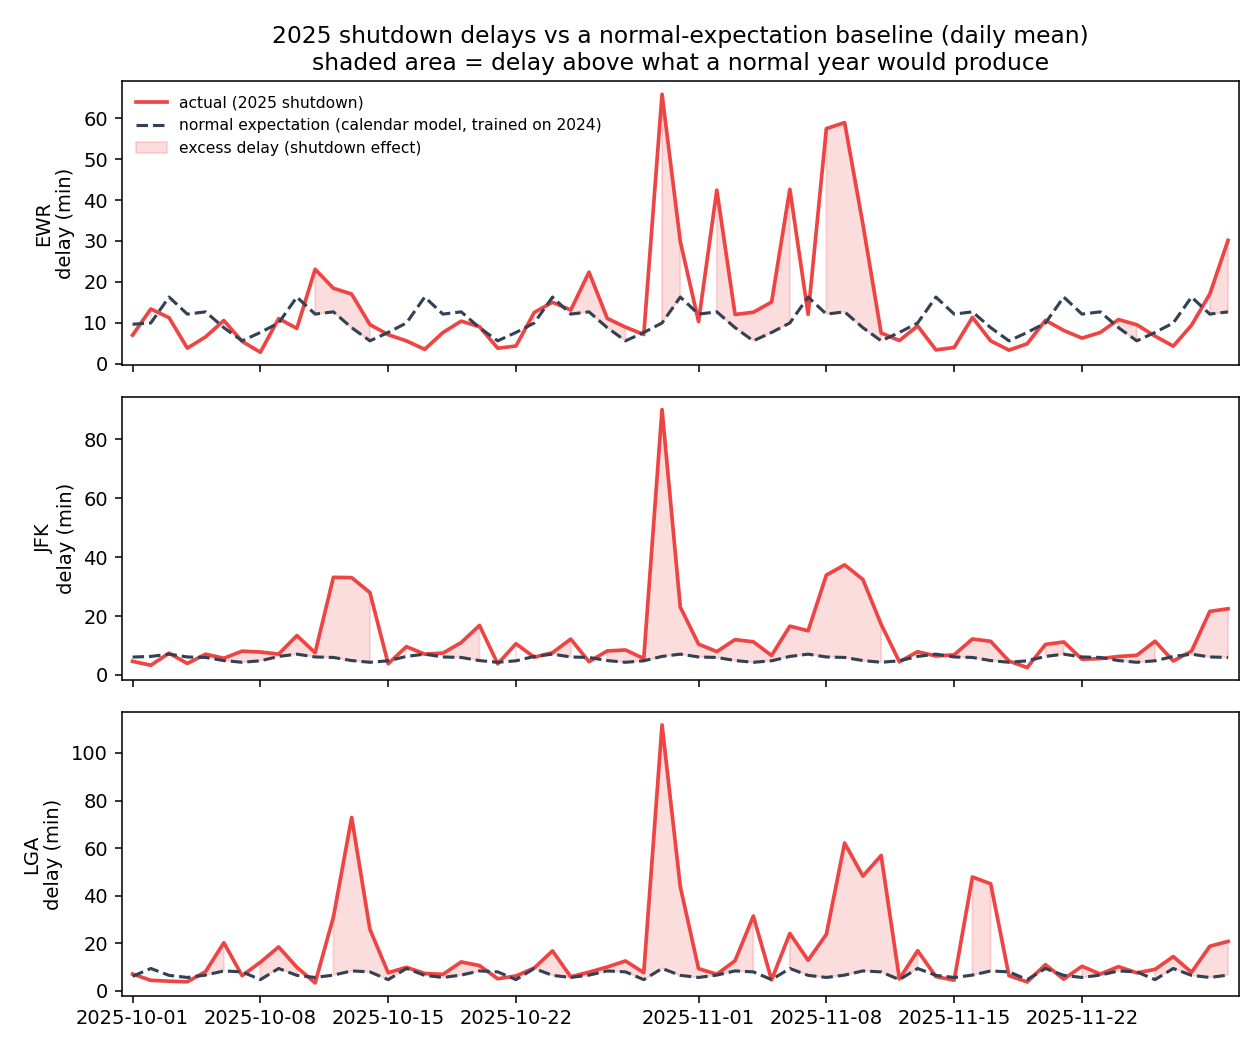
\includegraphics[width=0.9\linewidth]{shutdown_pred_vs_actual.png}
\caption{Actual daily mean delay during the 2025 shutdown (red) vs.\ the
normal-expectation counterfactual (dashed). The shaded area is the
shutdown-attributable excess.}
\label{fig:counterfactual}
\end{figure*}

\subsection{Leakage-Free Forecast of the Disruption}
\label{sec:res-forecast}
Table~\ref{tab:forecast} reports the strict, leakage-free forecast of November
2025. The shutdown-aware model beats climatology on $R^2$ at all three
airports, and on MAE at EWR and LGA. At JFK the model's MAE is marginally worse
(9.5 vs.\ 9.3 minutes) even though its $R^2$ is far better: it captures the
high-delay disruption hours (which dominate squared error) at the cost of
slightly larger typical-hour errors. Figure~\ref{fig:forecast} overlays the
forecasts, actuals, and climatology.

\begin{table}[!t]
\centering
\small
\caption{Leakage-free forecast of November 2025 airport-hour delays.
Climatology is the 2024 hour$\times$day-of-week mean.}
\label{tab:forecast}
\begin{tabular}{lcccc}
\toprule
Airport & $R^2$ model & $R^2$ clim. & MAE model & MAE clim. \\
\midrule
EWR & \textbf{0.229} & 0.088 & \textbf{12.4} & 12.9 \\
JFK & \textbf{0.119} & $-0.005$ & 9.5 & \textbf{9.3} \\
LGA & \textbf{0.153} & $-0.042$ & \textbf{15.2} & 15.7 \\
\bottomrule
\end{tabular}
\end{table}

\begin{figure*}[!t]
\centering
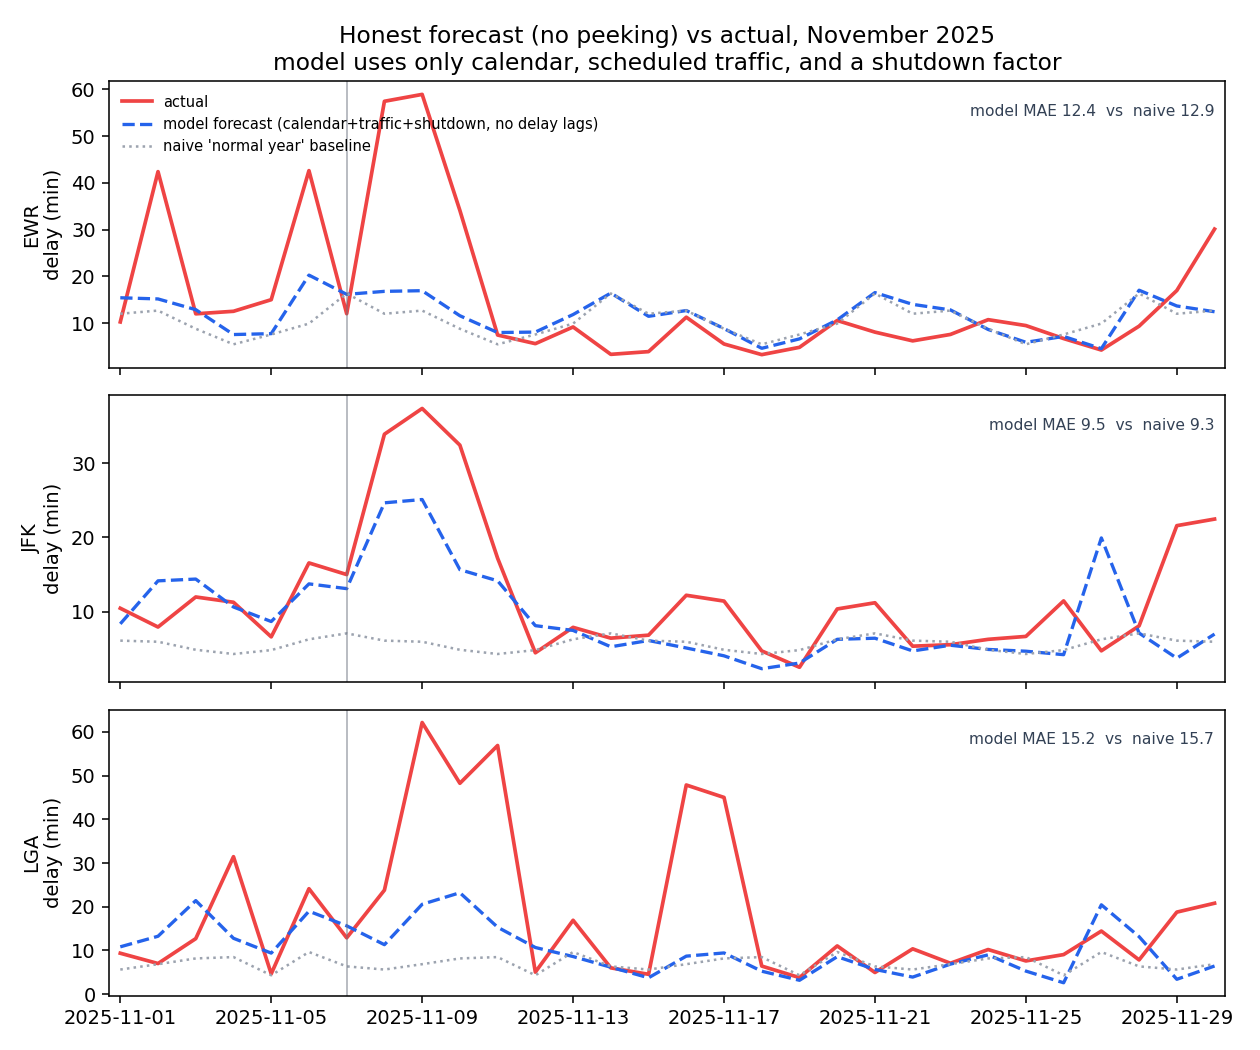
\includegraphics[width=0.9\linewidth]{shutdown_predict_vs_actual.png}
\caption{Leakage-free forecasts (blue dashed) vs.\ actual daily mean delay
(red) and the naive normal-year climatology (gray dotted), November 2025. The
vertical line marks the FAA flight-cut order taking effect.}
\label{fig:forecast}
\end{figure*}

\subsection{State-Dependent Delay Coupling}
\label{sec:res-coupling}
In January 2023 (which contains the January~11 NOTAM outage and nationwide
ground stop \cite{icao2023notam}), the network model improves out-of-sample
$R^2$ from 0.215 to 0.351 at JFK and from 0.138 to 0.211 at LGA, while EWR
degrades slightly (0.097 to 0.071); lead--lag correlations identify Newark as
the upstream driver ($r=0.573$ and $0.565$ to JFK and LGA at $t{+}1$;
Figure~\ref{fig:evidence}). Repeating the identical design across regimes
(Table~\ref{tab:replication}) shows the coupling is not constant: the
EWR$\rightarrow$JFK lead--lag correlation is only $0.19$ in normal 2024 but
$0.55$ during the 2025 shutdown, comparable to the disrupted January 2023
month.

\begin{table}[!t]
\centering
\small
\caption{State-dependence of metro delay coupling. Top: EWR($t$)
$\rightarrow$ neighbor($t{+}1$) Pearson correlation. Bottom: change in
out-of-sample $R^2$ from adding corridor-neighbor features.}
\label{tab:replication}
\begin{tabular}{lccc}
\toprule
 & Jan 2023 & Oct--Nov 2024 & Oct--Nov 2025 \\
 & (NOTAM) & (normal) & (shutdown) \\
\midrule
$r$\,[EWR$\to$JFK($t{+}1$)] & 0.573 & 0.193 & 0.547 \\
$r$\,[EWR$\to$LGA($t{+}1$)] & 0.565 & 0.134 & 0.445 \\
$\Delta R^2$ JFK & $+0.135$ & $+0.110$ & $+0.015$ \\
$\Delta R^2$ LGA & $+0.072$ & $-0.198$ & $-0.206$ \\
$\Delta R^2$ EWR & $-0.025$ & $+0.025$ & $+0.023$ \\
\bottomrule
\end{tabular}
\end{table}

\begin{figure}[!t]
\centering
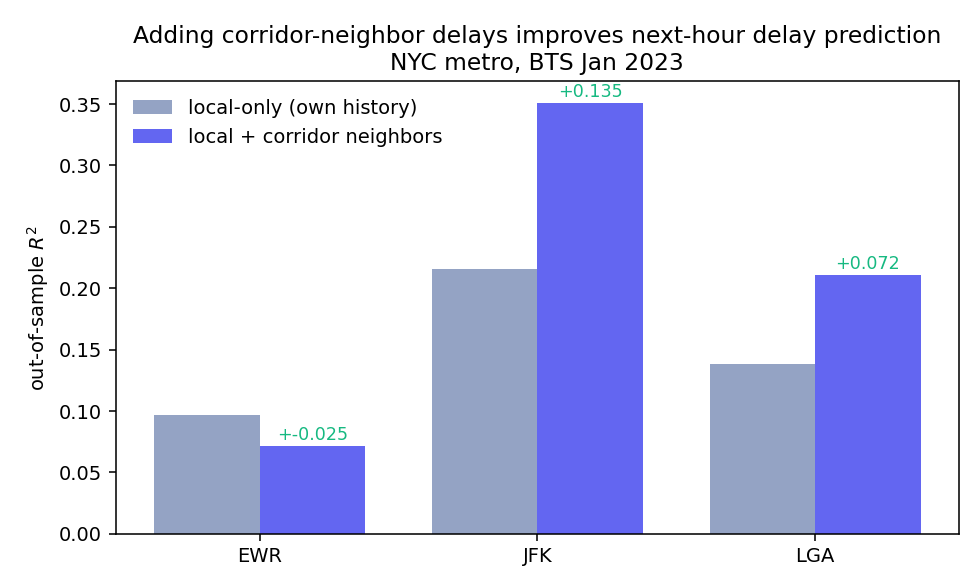
\includegraphics[width=\linewidth]{evidence_r2.png}
\caption{January 2023: adding corridor-neighbor delays improves next-hour
prediction for the downstream hubs (JFK, LGA) but not the upstream driver
(EWR).}
\label{fig:evidence}
\end{figure}

% =====================================================================
\section{Discussion}
\label{sec:discussion}

\paragraph{How much did the shutdown cost the NYC metro?}
The three counterfactuals converge on roughly 0.40--0.42 million excess
departure-delay-minutes, about \$41M in direct operating cost at three airports
over two months (Table~\ref{tab:excess}), and weather does not explain it,
consistent with the Richmond Fed's weather-controlled national estimate
\cite{richmondfed2025}. This figure is a conservative lower bound: it counts
only delay-minutes of \emph{operated} flights, while cancellations rose three-
to eight-fold (Table~\ref{tab:cancel}), removing the worst potential delays
from the sample entirely. The headline effect is carried by JFK and LGA, whose
increases are highly significant; Newark's smaller, non-significant rise
reflects its heavy, volatile baseline rather than an absence of impact. For
scale, our local \$41M sits comfortably inside the national picture: a
$\sim$\$66M nationwide estimate of delay labor-hours measured on a different
basis \cite{richmondfed2025}, and a multi-billion-dollar total economic impact
including cancellations and passenger time \cite{ctp2026}.

\paragraph{Could it have been forecast?}
Yes, in the operationally meaningful sense. A model that uses only information
available in advance (calendar, scheduled traffic, and the public fact that a
shutdown is in effect) beats a normal-year climatology at all three airports
(Table~\ref{tab:forecast}). The absolute $R^2$ values are modest because hourly
delay under an unprecedented disruption is genuinely hard to predict from
calendar-level features; the point is comparative. A model that merely ``knows a
shutdown is underway'' anticipates a meaningful share of the disruption that a
normal-year model misses entirely. This matters because the
alternative, using recent realized delays, amounts to reacting rather than
forecasting; our strict leakage-free protocol shows real anticipatory signal
without that crutch.

\paragraph{Why the delay network changes under stress}
During large disruptions the metro behaves as a strongly coupled directed
system with Newark upstream; in normal operations the airports are closer to
independent and local history dominates (Table~\ref{tab:replication}). This has
two consequences. Methodologically, single-period evaluations of graph
models (common in the literature, and true of our own January 2023 analysis
had we stopped there) can over- or under-state the value of network structure
depending on the regime sampled. Operationally, it is precisely when the system
is disrupted, when intervention decisions matter most, that network information
carries signal, which motivates disruption-conditional graph models rather than
static ones.

\subsection{Limitations}
\label{sec:limitations}
\textbf{Departures only.} We measure departure delay at three airports;
arrival delays, diversions, and downstream national effects are out of scope.
\textbf{Cost basis.} The \$100.76/block-minute figure is a direct airline
operating cost; it excludes passenger time and cancellation costs, so our
dollar figures are conservative lower bounds on social cost.
\textbf{Counterfactual assumptions.} The model counterfactual clips negative
hourly excess at zero (delay prevented by the FAA's own traffic cuts is not
netted out); the prior-year baseline assumes 2024 is a valid normal. Their
agreement (and the weather adjustment) mitigates but does not eliminate this.
\textbf{Panel construction.} Hours with no scheduled departures are zero-filled,
slightly attenuating overnight dynamics.
\textbf{Two-year comparison.} A full difference-in-differences with control
airports (as in \cite{richmondfed2025}) would strengthen identification; our
convergent-counterfactual design is the single-metro analogue.
\textbf{Coupling analysis.} The state-dependence finding rests on three
periods; a systematic scan over many months and disruption events is the
natural next step.

% =====================================================================
\section{Conclusion and Future Work}
\label{sec:conclusion}
Using only public data, we measured what the 2025 government shutdown did to
the New York metro's departures: significant delay increases at JFK (+107\%)
and LGA (+149\%), a three- to eight-fold rise in cancellations, and
0.40--0.42 million excess delay-minutes ($\approx$\,\$41M in direct operating
cost) that three independent counterfactuals agree on and weather does not
explain. A forecasting model that merely knows a shutdown is underway
anticipates a meaningful part of the disruption ahead of time. And the metro's
delay network itself changes under stress: inter-airport coupling that is weak
in normal operations triples during disruptions. Together these results provide
a reproducible local complement to national estimates of the shutdown's cost
and an empirical foundation for disruption-aware models of the airspace.

\paragraph{Future work}
The state-dependent coupling result sharpens the case for graph models that
reason about \emph{interventions}, not just predictions. The FAA's blanket
flight reductions were criticized as blunt \cite{ctp2026}; choosing \emph{where} and
\emph{when} to hold traffic is a counterfactual question that observational
models, including Granger-causal ones \cite{zhu2024}, cannot answer. Our
planned next step is a simulation-augmented spatio-temporal GNN: a lightweight
Northeast-corridor simulator generates (baseline, intervention, outcome)
triples, and a GNN with an intervention head is trained jointly on real BTS
data and simulated counterfactuals, following treatment-effect estimation
practice \cite{shi2019}. The measurements in this paper supply its evaluation
targets: the shutdown excess (Table~\ref{tab:excess}), the NOTAM-outage month,
and the disruption-conditional coupling structure (Table~\ref{tab:replication}).

\paragraph{Reproducibility}
All analyses use public BTS on-time files and IEM METAR archives; the full
pipeline (data loading, panels, models, tables, and figures) is a small set of
Python scripts run end-to-end with fixed random seeds.

\bibliographystyle{IEEEtran}
\bibliography{references}

\end{document}
